\section{Evaluation}

 \frame{\sectionpage}

\begin{frame}{Shock of Surprising Reverses}

    \begin{table}[h!]
        \small
        \begin{center}
          \begin{tabular}{lcc}
            
             & Predicted denial & Predicted success  \\
            \hline
            Actual denial & \only<2->{affirm and predicted affirm} & \only<2->{affirm but predicted reverse}\\
            Actual success & \only<3->{\color{goldenrod}reverse but predicted affirm} & \only<2->{reverse and predicted reverse}
          \end{tabular}
        \end{center}
      \end{table}

    \uncover<4->{
        \begin{itemize}
            \item<4-> reverse: denial asylum in the lower court, but grant asylum in the appeal court
            \item<5-> \textbf{\color{goldenrod}surprising reverse}: predicted affirm, but actually reversed
        \end{itemize}
    }
    
\end{frame}

\begin{frame}{Interpretation: Estimation}
    \begin{columns}

        \begin{column}{0.45\textwidth}
            \begin{figure}
            \centering
            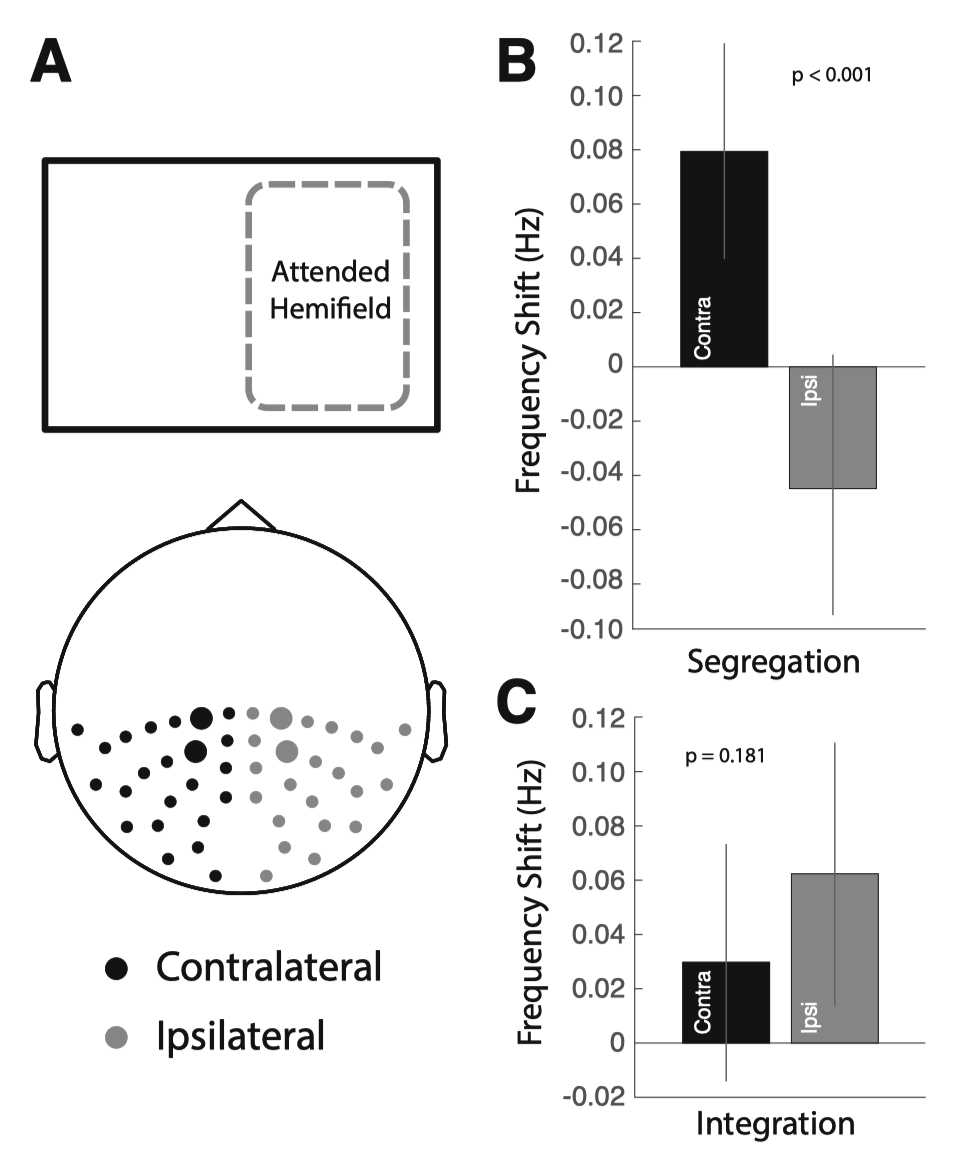
\includegraphics[height = 0.75 \textheight]{images/res4_1.png}
            \end{figure}
        \end{column}
        
        \begin{column}{0.55\textwidth}
    
        \only<2->{
            neutral-cue as baseline\uncover<3->{: like adding \textcolor{lightlavender}{\textbf{{task FE}}}}
            {\begin{itemize}\small
                \item<4-> driven by contralateral cortex itself
                \item<5-> opposite effects on contralateral and ipsilateral cortex
            \end{itemize}}
            }
        
        \end{column}
        \end{columns}
\end{frame}

\begin{frame}{Interpretation: the Role of Spatial Attention}
    \begin{columns}

        \begin{column}{0.6\textwidth}
            \begin{figure}
            \centering
            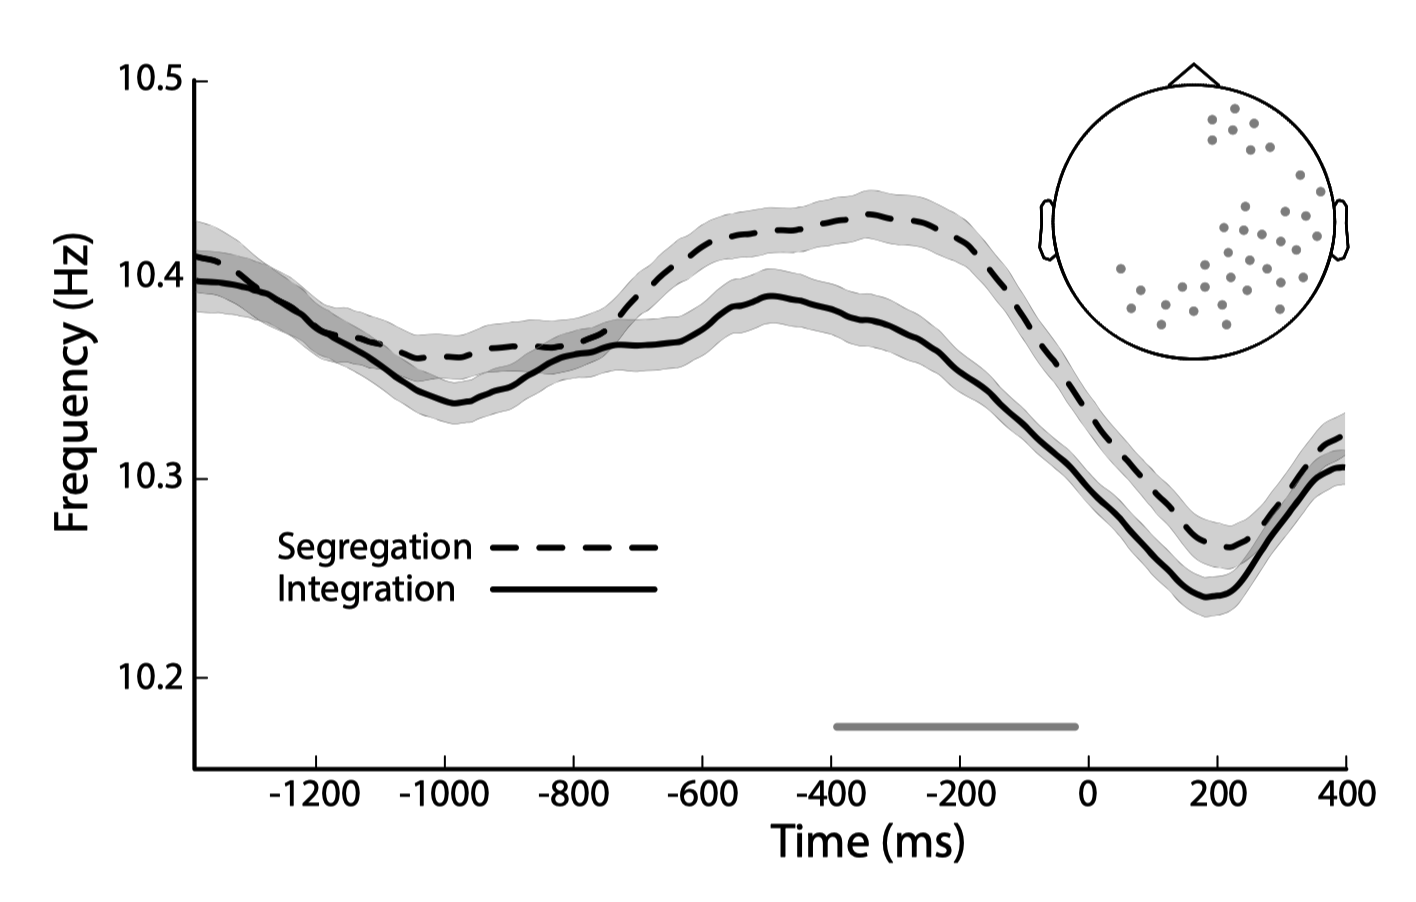
\includegraphics[height = 0.7 \textheight]{images/res3_1.png}
            \end{figure}
        \end{column}
        
        \begin{column}{0.35\textwidth}
    
        \only<2->{
            There is a difference under neutral cues:
            \begin{itemize}\small
                \item<2-> temporal visual processing is \textcolor{lightlavender}{\textbf{itself}} sentitive to strategic preparation
                \item<3-> spatial attention does \textcolor{lightlavender}{\textbf{accentuate}} this broader influence
            \end{itemize}
            }
        
        \end{column}
        \end{columns}
    
\end{frame}

\begin{frame}{Interpretation: Understanding $\alpha$}
    \begin{columns}

        \begin{column}{0.45\textwidth}
            \begin{figure}
            \centering
            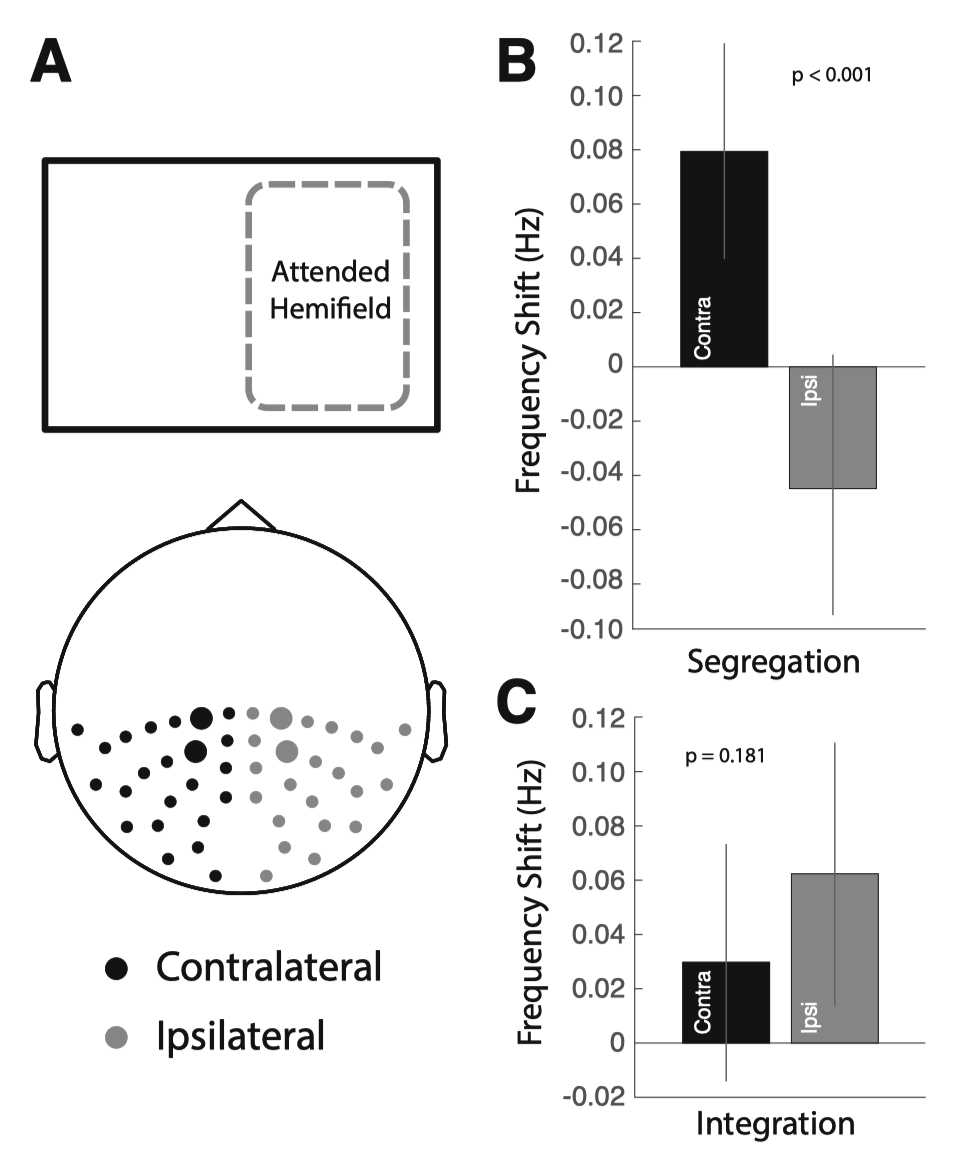
\includegraphics[height = 0.75 \textheight]{images/res4_1.png}
            \end{figure}
        \end{column}
        
        \begin{column}{0.55\textwidth}
    
        \only<2->{
            
            {\begin{itemize}\small
                \item<2-> more salient effects for \textcolor{lightlavender}{\textbf{{segragation}}}: 
                
                increase in contralateral $\alpha$ is \textcolor{lightlavender}{\textbf{{associated}}} with perceptual sensitivity in the detection of fleeting visual stimuli {\scriptsize(See \citet{di2022tuning})}
                \item<3-> $\alpha$ relects \textcolor{lightlavender}{\textbf{{rhythmic inhibition}}}: 
                
                spatial attention {\footnotesize(or the deployment of attention in general)} can flexibly \textcolor{lightlavender}{\textbf{{adapt}}} oscillatory activity to strategically \textcolor{lightlavender}{\textbf{{optimize}}} the time duration that fits in the \textit{open} portion of an $\alpha$ cycle
            \end{itemize}}
            }
        
        \end{column}
        \end{columns}
    
\end{frame}